
\chapter{Prediction System}
The main goal during this phase was to find a way to implement a forecast system in Python.
Since the datasets used during this thesis could be considered as a time series, was decide to implement and test an Autoregressive Integrated Moving Average (ARIMA) model. \\
Since there are several possible configurations for fit an ARIMA model, is important to find the right one to use with each input dataset because it would allows to have much better prediction results.
In order to find the best ARIMA configuration there are different methods and procedure, like one of the most known that is "Box–Jenkins method"\footnote{Check out the Box–Jenkins method at the current link: \\ \url{https://en.wikipedia.org/wiki/Box\%E2\%80\%93Jenkins_method}}. In this study was decied to use an easier method, in order to have a first approach with this system and a general idea about the problem. It basically consists in testing different ARIMA model configurations for the same input dataset and then check the results.\\
For this reason during this phase of the work have been implemented 2 different subsytems for two different purposes:
\begin{enumerate}
\item Evaluating System
\item Prediction System
\end{enumerate}

\newpage
\section{Evaluating System}
\textbf{Goal:}\\ 
Used for evaluate different configurations of ARIMA machine. \\ It tests 112 different configurations for the current input that we would like to forecast and report the results with each MAPE (Mean Average Percentage Error) values.

\textbf{Requirements:}\\
There are not any kind of needed requirements. It's possible to use this system on dataset of arbitrary length.

\textbf{Code implementation:}\\
This time the full commented code has not been reported in the appendice since is longer and more complicated than the previous. If you are interested to check out more details about the code, is possible to find the Github repository here : [\ref{Repository}]

The most important part of the code about the Evaluating System is the following.\\
Basically the method ARIMA() allows to train a model based on historic values (history) and a specific order (p,d,q). After that it's possible to call the method forecast() through the trained model and having some predictions like result.
\begin{lstlisting}
model = ARIMA(history, order=arima_order)
model_fit = model.fit(disp=0)
yhat = model_fit.forecast()[0]
\end{lstlisting}

More in the specific, the 112 different ARIMA configurations that were tested are all the possible combinations between the following three parameters values:
\begin{lstlisting}
p_values = [0, 1, 2, 4, 6, 8, 10]
d_values = [0, 1, 2, 3]
q_values = [0, 1, 2, 3]
\end{lstlisting}

\newpage

\textbf{Results:}\\
The system will display the MAPE between real value and predicted values for each of the 112 tested ARIMA machine. In particular, once tested all the configurations, the system will provide the configuration that gave the best MAPE result.\\
All these results have been reported in a document that is possible to check for check out the different configurations result.

The following graphic display the different ARIMA configurations tested, providing also:
\vspace{-5mm}
\begin{itemize}
 \setlength{\itemsep}{-5pt} 
\item General overview about MAPE values for each single tested configuratons. 
\item Best configuration with relative MAPE value.
\item Color legend, where the red means lower MAPE, so more accurate predictions, and blue means higher MAPE, so less accurate predictions.
\end{itemize}

\begin{figure}[H]
	\raggedleft
	\makebox[1\textwidth][c]{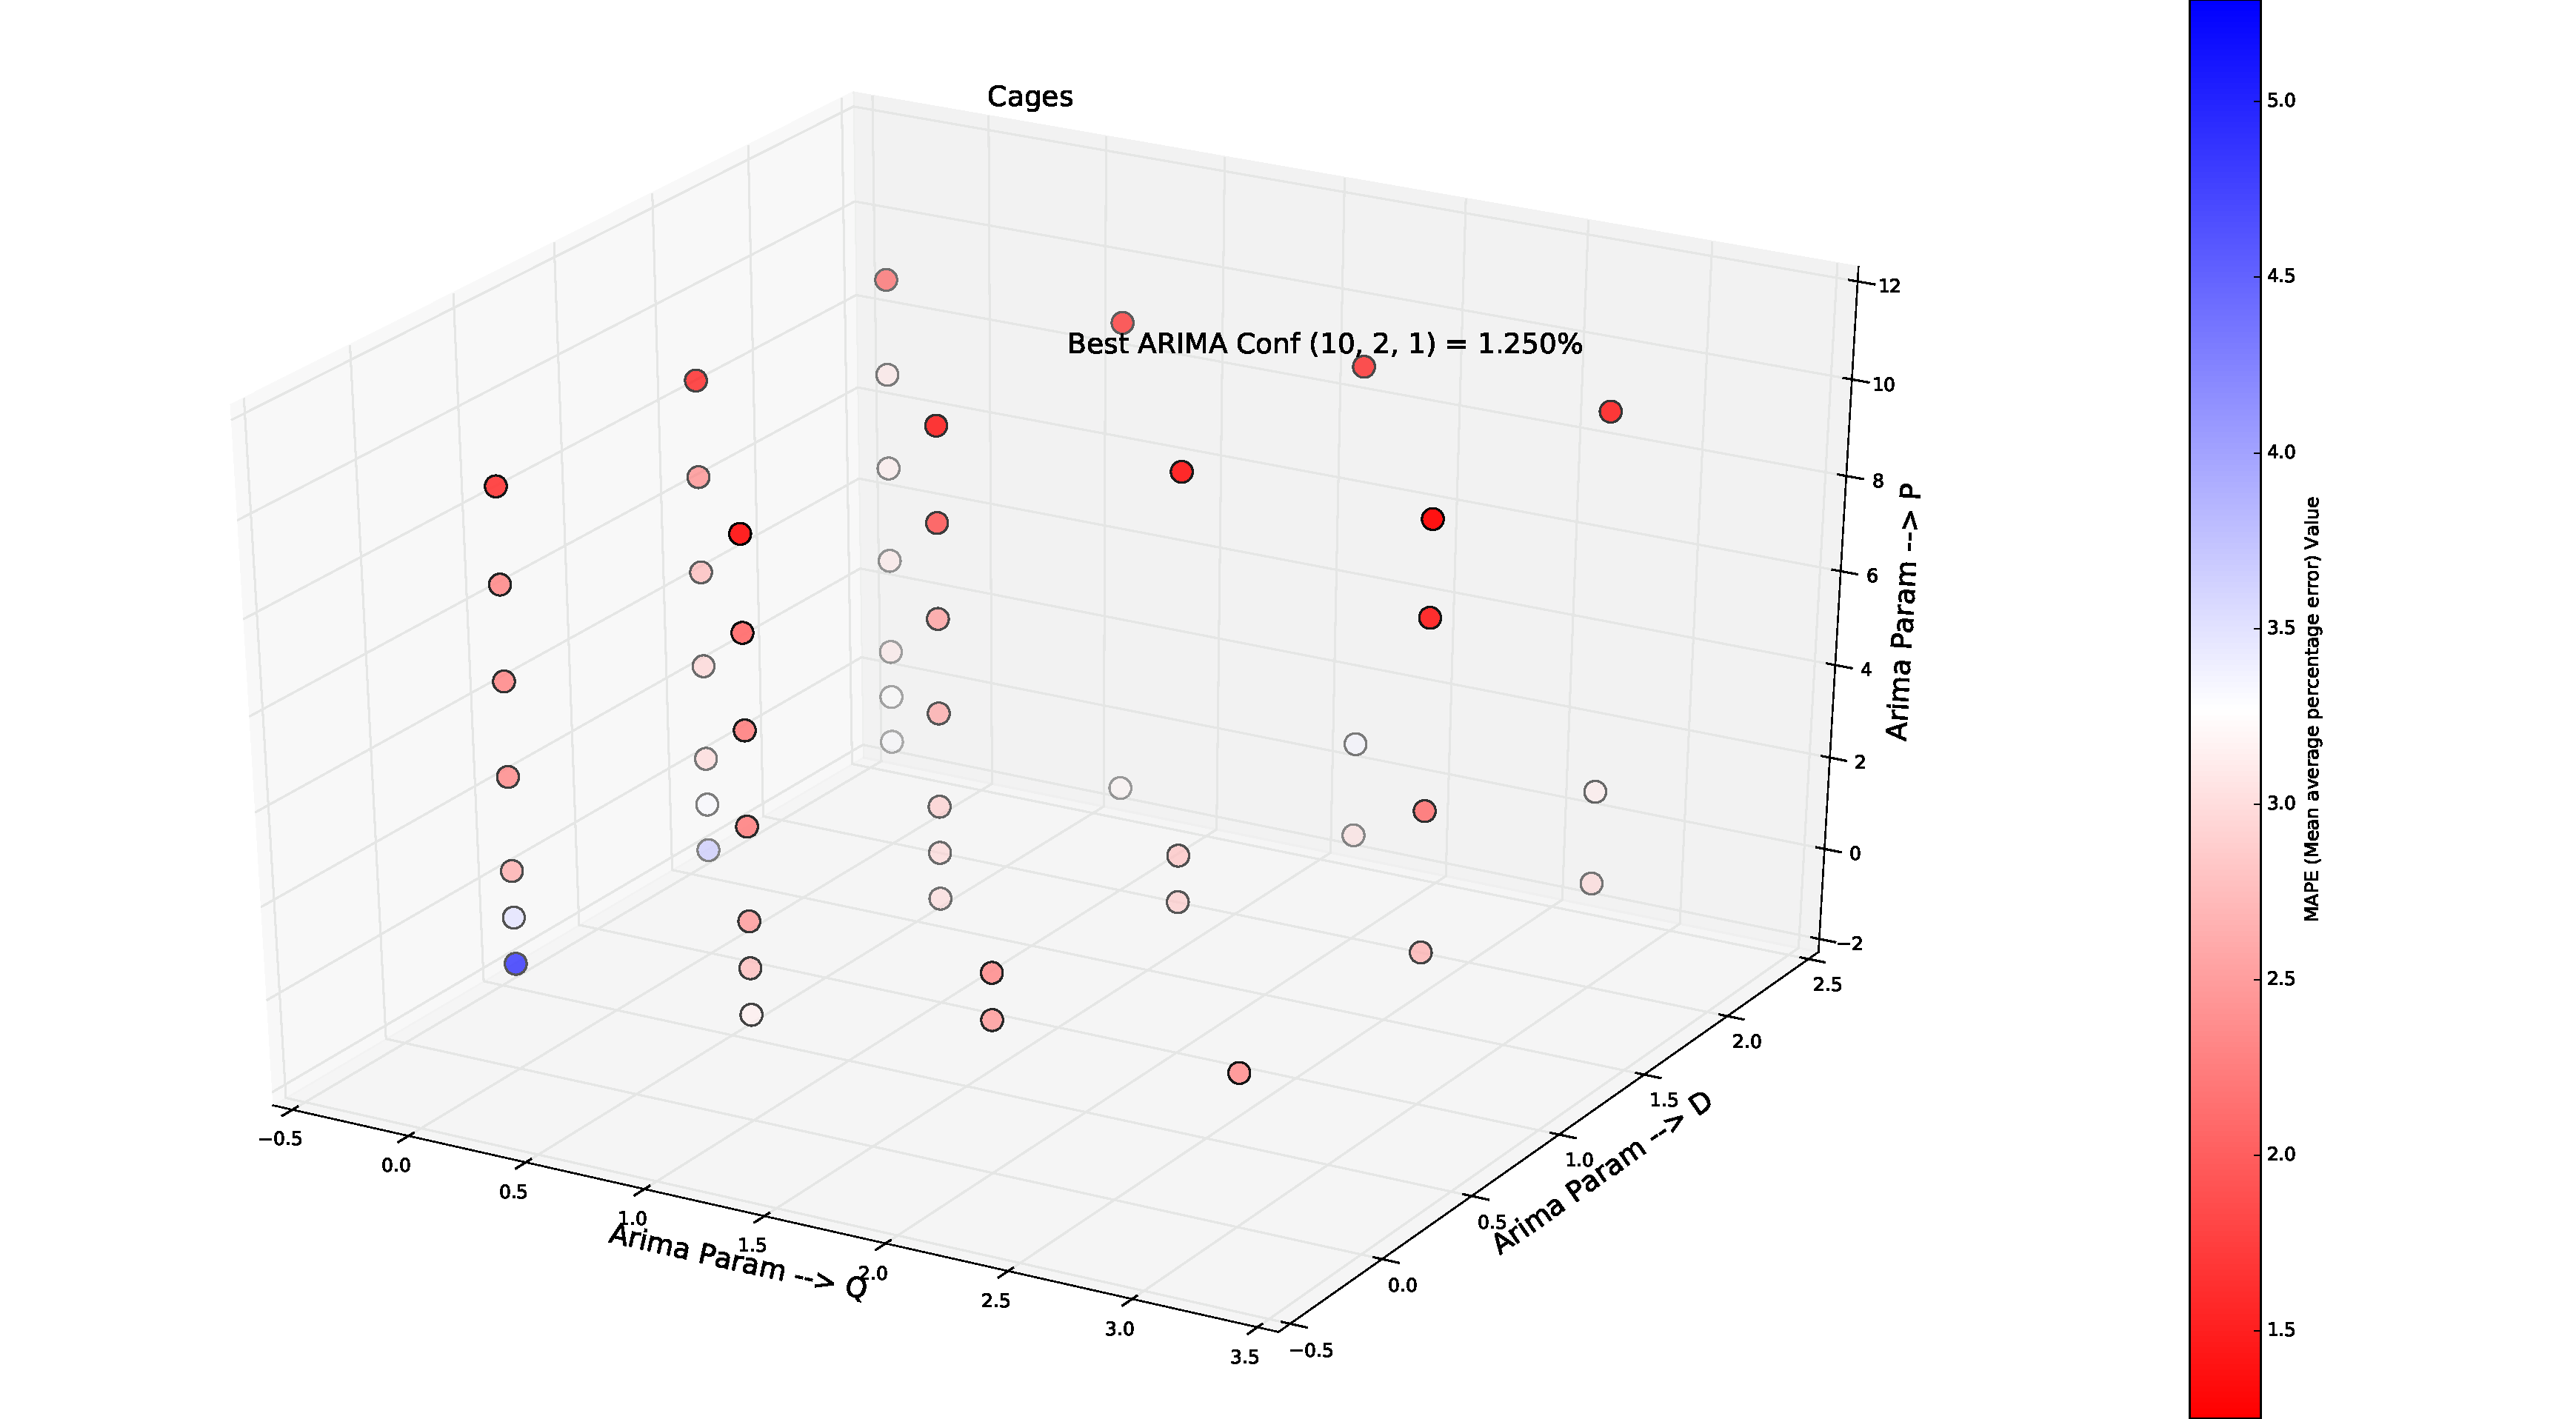
\includegraphics[width=1.5\textwidth]{Files/Cages_MAPE.pdf}}
    \caption{Graphic that displays different MAPE values for each ARIMA order.}
\end{figure}

 
 
\newpage
\section{Prediction System}
\textbf{Goal:}\\ 
This system has three main goals:
\vspace{-5mm}
\begin{itemize}
 \setlength{\itemsep}{-5pt} 
\item Testing a specific ARIMA configuration on a particular data input, and display how much accurate it is (MAPE).
\item Predict some future value with the same ARIMA configuration.
\item Display the historic data together with the testing and future predictions.
\end{itemize}

\textbf{Requirements:}\\
There are not any kind of needed requirements. It's possible to use this system on input dataset of arbitrary length.


\textbf{Code implementation:}\\
To reach the first of the goals reported above the system will divide the input dataset in two parts, train and test. It allows to train the ARIMA model with just the "train" part of the dataset, that usually is 66\% of the whole dataset, and then try to predict the rest of the dataset values, comparing in the end with the values contain in the "test" part to have a general idea about the accuracy.

The method ARIMA() allows to train a model based on historic values (history) and a specific order (p,d,q). After that it's possible to call the method forecast() through the trained model and having some predictions like result.

\begin{lstlisting}
model = ARIMA(history, order=arima_order)
model_fit = model.fit(disp=0)
yhat = model_fit.forecast()[0]
\end{lstlisting}

Then the system will also predict a number of future values choosen by the system user.
\begin{lstlisting}
model = ARIMA(dataset, order=order)
model_fit = model.fit(disp=0)
forecast = model_fit.forecast(int(sys.argv[3]))[0]
\end{lstlisting}

The final step is to display the historic data together with the test prediction and the future prediction on the same graphic. 
\begin{lstlisting}
# Plot current input's historic values 
series.plot(color="blue", linewidth=1.5, label="Series: "+sys.argv[1])

# Plot current input's test prediction
predHistoric.plot(color="red", linewidth=1.5, label="Prediction test:")

# Plot current input's future prediction
predFuture.plot(color="green", linewidth=1.5, label="Future Prediction:")
\end{lstlisting}

This time the full commented code has not been reported in the appendice since is longer and more complicated than the previous. If you are interested to check out more details about the code, is possible to find the Github repository here : [\ref{Repository}]

\textbf{Results:}\\
This system will automatically generate two documents that contain:
\vspace{-5mm}
\begin{itemize}
 \setlength{\itemsep}{-5pt} 
\item Test predictions values
\item Future predictions values
\end{itemize}

And then it provides also the possibility to visualize the historic, test and future predictions values on the same graphic, that looks like the following example:

\begin{figure}[H]
    \makebox[\textwidth][c]{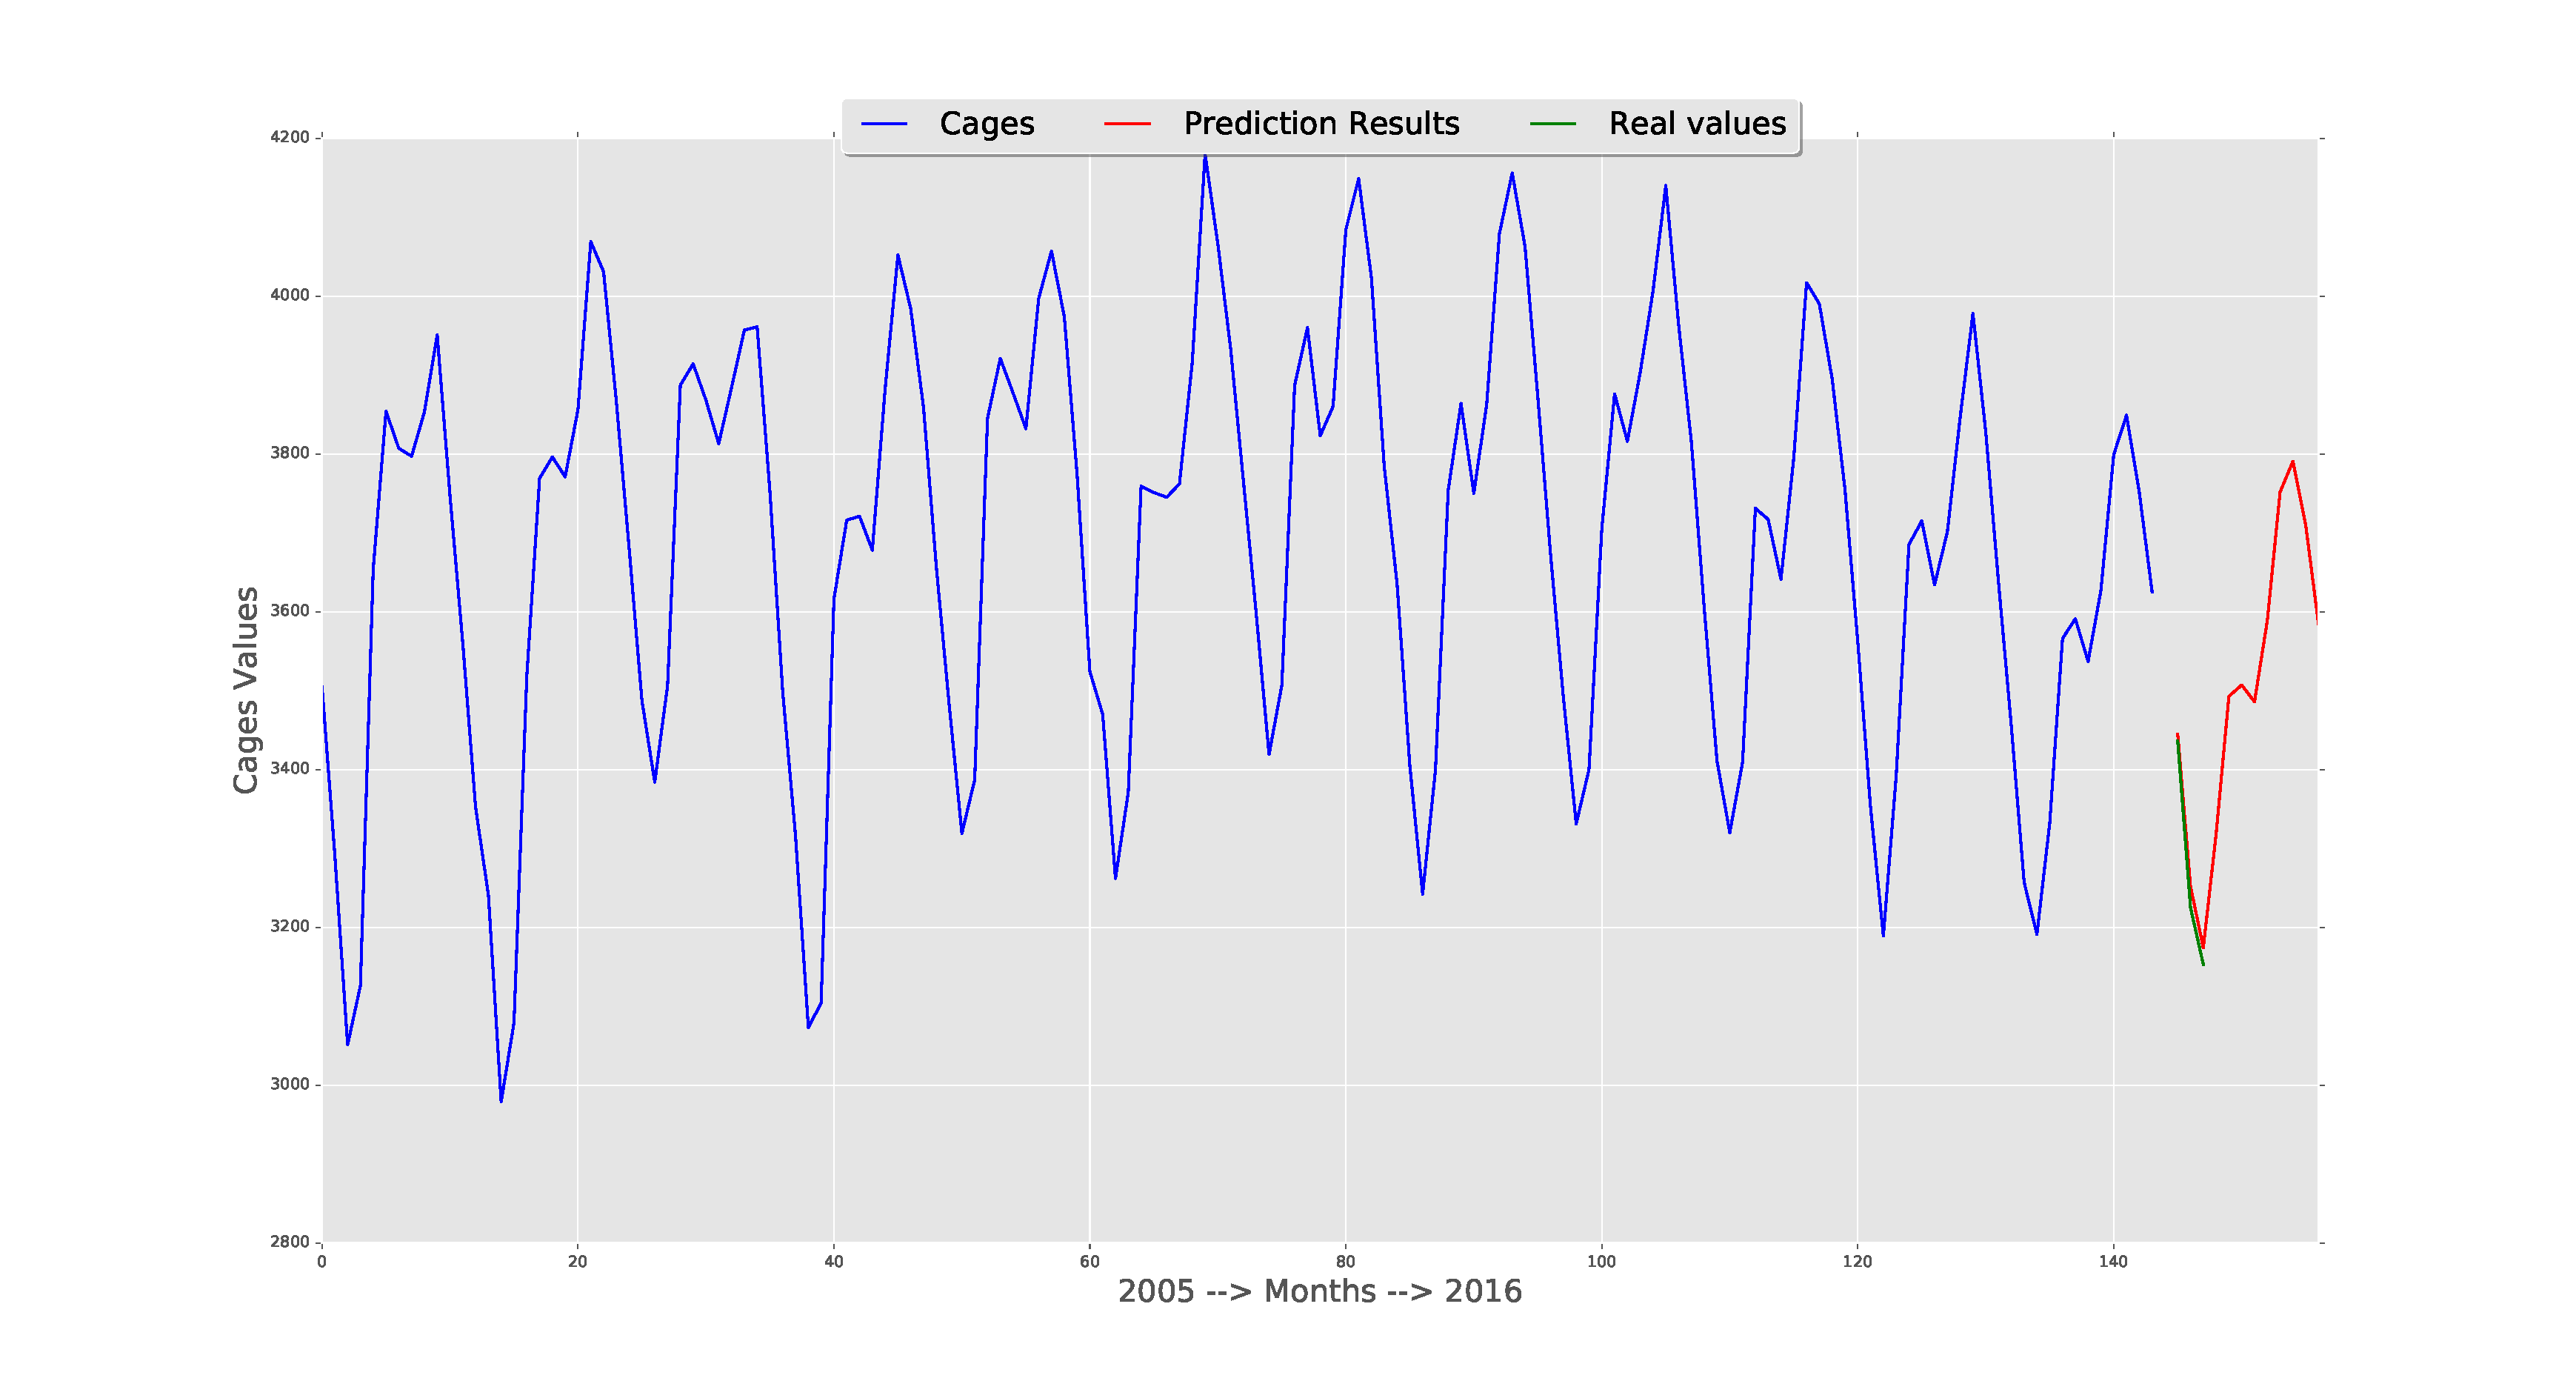
\includegraphics[width=1.5\textwidth]{Files/Cages_Predictions.pdf}}
    \caption{Graphic that display historic, future and predicted values of a input.}
\end{figure}


\newpage



